% Paper-friendly system architecture diagram (revised/delivered design only).
% Redesigned per .agents/rules/61-tikz-flow-diagrams.agents.md: Supabase and the
% Intelligence Service are two separate branches off the Client (left lane vs.
% down lane) so they never sit adjacent to each other.
% Standalone -> tight-bbox vector PDF. Compile: pdflatex fig_architecture.tex
\documentclass[border=6pt]{standalone}
\usepackage[T1]{fontenc}
\usepackage{helvet}
\renewcommand{\familydefault}{\sfdefault}
\usepackage{tikz}
\usetikzlibrary{positioning,fit,backgrounds,arrows.meta,shapes.geometric,calc}

\definecolor{blueStroke}{HTML}{1D4ED8}
\definecolor{blueFill}{HTML}{EFF6FF}
\definecolor{purpStroke}{HTML}{6D28D9}
\definecolor{purpFill}{HTML}{FAF5FF}
\definecolor{slate}{HTML}{475569}
\definecolor{slateFill}{HTML}{F1F5F9}
\definecolor{grey}{HTML}{9CA3AF}
\definecolor{greyFill}{HTML}{F2F2F2}
\definecolor{greyText}{HTML}{6B7280}
\definecolor{amber}{HTML}{B45309}
\definecolor{inkText}{HTML}{1F2937}

\begin{document}
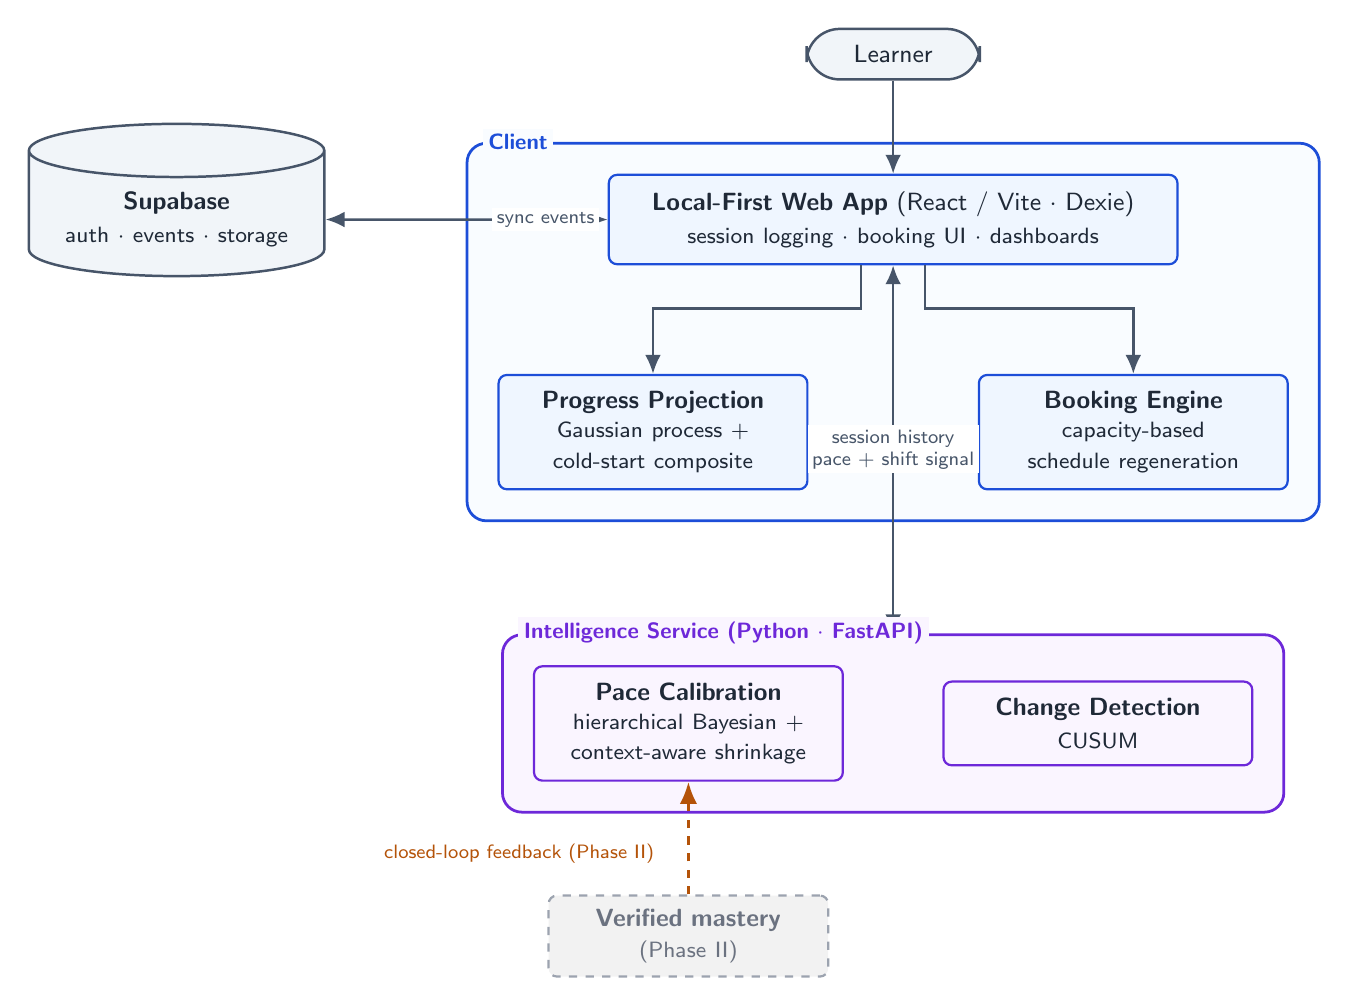
\begin{tikzpicture}[
  font=\small,
  every node/.style={text=inkText},
  box/.style={rounded corners=3pt, draw, line width=0.8pt, align=center,
              inner sep=6pt, text width=3.5cm, fill=white},
  proc/.style={box, draw=blueStroke, fill=blueFill},
  svc/.style={box, draw=purpStroke, fill=purpFill},
  hub/.style={cylinder, shape border rotate=90, aspect=0.18, draw=slate,
              line width=0.9pt, fill=slateFill, align=center, inner sep=5pt,
              text width=3.4cm, minimum height=1.3cm},
  actor/.style={rounded corners=12pt, draw=slate, line width=0.9pt,
                fill=slateFill, align=center, inner sep=6pt, minimum width=2.2cm},
  phase2/.style={rounded corners=3pt, draw=grey, dashed, line width=0.8pt,
                 fill=greyFill, text=greyText, align=center, inner sep=5pt, text width=3.2cm},
  title/.style={font=\footnotesize\bfseries},
  flow/.style={-{Latex[length=2.4mm,width=2.0mm]}, line width=0.9pt, draw=slate},
  flowbi/.style={{Latex[length=2.4mm,width=2.0mm]}-{Latex[length=2.4mm,width=2.0mm]},
                 line width=0.9pt, draw=slate},
  loop/.style={-{Latex[length=2.8mm,width=2.2mm]}, line width=1.1pt, dashed, draw=amber},
  lbl/.style={font=\scriptsize, fill=white, inner sep=1.6pt, text=slate, align=center},
  amblbl/.style={font=\scriptsize, fill=white, inner sep=1.6pt, text=amber},
]

% ---------------- NODES (absolute grid, cm) ----------------
% Spine at x=2: Learner -> App -> (down the GP/Booking gap) -> Intelligence Service.
% Supabase branches off to the LEFT at the App's own height (separate lane;
% never adjacent to the Intelligence Service box below).
\node[actor] (LEARNER) at (2,9.5) {Learner};
\node[proc, text width=6.8cm] (APP) at (2,7.4)
  {\textbf{Local-First Web App} (React / Vite $\cdot$ Dexie)\\[1pt]
   \footnotesize session logging $\cdot$ booking UI $\cdot$ dashboards};
\node[proc] (GP) at (-1.05,4.7) {\textbf{Progress Projection}\\[1pt]\footnotesize Gaussian process $+$\\\footnotesize cold-start composite};
\node[proc] (ENG) at (5.05,4.7) {\textbf{Booking Engine}\\[1pt]\footnotesize capacity-based\\\footnotesize schedule regeneration};

\node[hub] (SB) at (-7.1,7.4) {\textbf{Supabase}\\[1pt]\footnotesize auth $\cdot$ events $\cdot$ storage};

\node[svc] (CAL) at (-0.6,1.0) {\textbf{Pace Calibration}\\[1pt]\footnotesize hierarchical Bayesian $+$\\\footnotesize context-aware shrinkage};
\node[svc] (DET) at (4.6,1.0) {\textbf{Change Detection}\\[1pt]\footnotesize CUSUM};
\node[phase2] (V2) at (-0.6,-1.7) {\textbf{Verified mastery}\\\footnotesize(Phase II)};

% ---------------- CONTAINERS (background) ----------------
\begin{scope}[on background layer]
  \node[draw=blueStroke, line width=1pt, rounded corners=7pt, fill=blueFill!35,
        fit=(APP)(GP)(ENG), inner sep=11pt] (clientBox) {};
  \node[draw=purpStroke, line width=1pt, rounded corners=7pt, fill=purpFill,
        fit=(CAL)(DET), inner sep=11pt] (svcBox) {};
\end{scope}

% ---------------- EDGES ----------------
\draw[flow] (LEARNER) -- (APP);
\draw[flow] (APP.235) -- ++(0,-0.55) -| (GP.north);
\draw[flow] (APP.305) -- ++(0,-0.55) -| (ENG.north);
% Supabase: its own horizontal lane off the Client, well clear of the service box below.
\draw[flowbi] (APP.west) -- (SB.east) node[lbl, pos=0.22]{sync events};
% Intelligence Service: its own vertical lane, straight down the GP/Booking gap.
\draw[flowbi] (APP.south) -- (svcBox.north)
  node[lbl, pos=0.5]{session history\\pace $+$ shift signal};
% closed loop (Phase II)
\draw[loop] (V2.north) -- (CAL.south);
\node[amblbl] at (-2.75,-0.65) {closed-loop feedback (Phase II)};

% ---------------- CONTAINER TITLES (on top, after edges) ----------------
\node[title, text=blueStroke, fill=blueFill!35, inner sep=2pt, anchor=west]
      at ([xshift=6pt]clientBox.north west) {Client};
\node[title, text=purpStroke, fill=purpFill, inner sep=2pt, anchor=west]
      at ([xshift=6pt]svcBox.north west) {Intelligence Service (Python $\cdot$ FastAPI)};
\end{tikzpicture}
\end{document}
